
%% bare_conf.tex
%% V1.3
%% 2007/01/11
%% by Michael Shell
%% See:
%% http://www.michaelshell.org/
%% for current contact information.
%%
%% This is a skeleton file demonstrating the use of IEEEtran.cls
%% (requires IEEEtran.cls version 1.7 or later) with an IEEE conference paper.
%%
%% Support sites:
%% http://www.michaelshell.org/tex/ieeetran/
%% http://www.ctan.org/tex-archive/macros/latex/contrib/IEEEtran/
%% and
%% http://www.ieee.org/

%%*************************************************************************
%% Legal Notice:
%% This code is offered as-is without any warranty either expressed or
%% implied; without even the implied warranty of MERCHANTABILITY or
%% FITNESS FOR A PARTICULAR PURPOSE! 
%% User assumes all risk.
%% In no event shall IEEE or any contributor to this code be liable for
%% any damages or losses, including, but not limited to, incidental,
%% consequential, or any other damages, resulting from the use or misuse
%% of any information contained here.
%%
%% All comments are the opinions of their respective authors and are not
%% necessarily endorsed by the IEEE.
%%
%% This work is distributed under the LaTeX Project Public License (LPPL)
%% ( http://www.latex-project.org/ ) version 1.3, and may be freely used,
%% distributed and modified. A copy of the LPPL, version 1.3, is included
%% in the base LaTeX documentation of all distributions of LaTeX released
%% 2003/12/01 or later.
%% Retain all contribution notices and credits.
%% ** Modified files should be clearly indicated as such, including  **
%% ** renaming them and changing author support contact information. **
%%
%% File list of work: IEEEtran.cls, IEEEtran_HOWTO.pdf, bare_adv.tex,
%%                    bare_conf.tex, bare_jrnl.tex, bare_jrnl_compsoc.tex
%%*************************************************************************

% *** Authors should verify (and, if needed, correct) their LaTeX system  ***
% *** with the testflow diagnostic prior to trusting their LaTeX platform ***
% *** with production work. IEEE's font choices can trigger bugs that do  ***
% *** not appear when using other class files.                            ***
% The testflow support page is at:
% http://www.michaelshell.org/tex/testflow/



% Note that the a4paper option is mainly intended so that authors in
% countries using A4 can easily print to A4 and see how their papers will
% look in print - the typesetting of the document will not typically be
% affected with changes in paper size (but the bottom and side margins will).
% Use the testflow package mentioned above to verify correct handling of
% both paper sizes by the user's LaTeX system.
%
% Also note that the "draftcls" or "draftclsnofoot", not "draft", option
% should be used if it is desired that the figures are to be displayed in
% draft mode.
%
\documentclass[conference]{IEEEtran}
% Add the compsoc option for Computer Society conferences.
%
% If IEEEtran.cls has not been installed into the LaTeX system files,
% manually specify the path to it like:
% \documentclass[conference]{../sty/IEEEtran}
% Some very useful LaTeX packages include:
% (uncomment the ones you want to load)


% *** MISC UTILITY PACKAGES ***
%
%\usepackage{ifpdf}
% Heiko Oberdiek's ifpdf.sty is very useful if you need conditional
% compilation based on whether the output is pdf or dvi.
% usage:
% \ifpdf
%   % pdf code
% \else
%   % dvi code
% \fi
% The latest version of ifpdf.sty can be obtained from:
% http://www.ctan.org/tex-archive/macros/latex/contrib/oberdiek/
% Also, note that IEEEtran.cls V1.7 and later provides a builtin
% \ifCLASSINFOpdf conditional that works the same way.
% When switching from latex to pdflatex and vice-versa, the compiler may
% have to be run twice to clear warning/error messages.






% *** CITATION PACKAGES ***
%
%\usepackage{cite}
% cite.sty was written by Donald Arseneau
% V1.6 and later of IEEEtran pre-defines the format of the cite.sty package
% \cite{} output to follow that of IEEE. Loading the cite package will
% result in citation numbers being automatically sorted and properly
% "compressed/ranged". e.g., [1], [9], [2], [7], [5], [6] without using
% cite.sty will become [1], [2], [5]--[7], [9] using cite.sty. cite.sty's
% \cite will automatically add leading space, if needed. Use cite.sty's
% noadjust option (cite.sty V3.8 and later) if you want to turn this off.
% cite.sty is already installed on most LaTeX systems. Be sure and use
% version 4.0 (2003-05-27) and later if using hyperref.sty. cite.sty does
% not currently provide for hyperlinked citations.
% The latest version can be obtained at:
% http://www.ctan.org/tex-archive/macros/latex/contrib/cite/
% The documentation is contained in the cite.sty file itself.






% *** GRAPHICS RELATED PACKAGES ***
%
\ifCLASSINFOpdf
  \usepackage[pdftex]{graphicx}
  % declare the path(s) where your graphic files are
  % \graphicspath{{../pdf/}{../jpeg/}}
  % and their extensions so you won't have to specify these with
  % every instance of \includegraphics
  % \DeclareGraphicsExtensions{.pdf,.jpeg,.png}
\else
  % or other class option (dvipsone, dvipdf, if not using dvips). graphicx
  % will default to the driver specified in the system graphics.cfg if no
  % driver is specified.
  \usepackage[dvips]{graphicx}
  % declare the path(s) where your graphic files are
  % \graphicspath{{../eps/}}
  % and their extensions so you won't have to specify these with
  % every instance of \includegraphics
  % \DeclareGraphicsExtensions{.eps}
\fi
% graphicx was written by David Carlisle and Sebastian Rahtz. It is
% required if you want graphics, photos, etc. graphicx.sty is already
% installed on most LaTeX systems. The latest version and documentation can
% be obtained at: 
% http://www.ctan.org/tex-archive/macros/latex/required/graphics/
% Another good source of documentation is "Using Imported Graphics in
% LaTeX2e" by Keith Reckdahl which can be found as epslatex.ps or
% epslatex.pdf at: http://www.ctan.org/tex-archive/info/
%
% latex, and pdflatex in dvi mode, support graphics in encapsulated
% postscript (.eps) format. pdflatex in pdf mode supports graphics
% in .pdf, .jpeg, .png and .mps (metapost) formats. Users should ensure
% that all non-photo figures use a vector format (.eps, .pdf, .mps) and
% not a bitmapped formats (.jpeg, .png). IEEE frowns on bitmapped formats
% which can result in "jaggedy"/blurry rendering of lines and letters as
% well as large increases in file sizes.
%
% You can find documentation about the pdfTeX application at:
% http://www.tug.org/applications/pdftex





% *** MATH PACKAGES ***
%
%\usepackage[cmex10]{amsmath}
% A popular package from the American Mathematical Society that provides
% many useful and powerful commands for dealing with mathematics. If using
% it, be sure to load this package with the cmex10 option to ensure that
% only type 1 fonts will utilized at all point sizes. Without this option,
% it is possible that some math symbols, particularly those within
% footnotes, will be rendered in bitmap form which will result in a
% document that can not be IEEE Xplore compliant!
%
% Also, note that the amsmath package sets \interdisplaylinepenalty to 10000
% thus preventing page breaks from occurring within multiline equations. Use:
%\interdisplaylinepenalty=2500
% after loading amsmath to restore such page breaks as IEEEtran.cls normally
% does. amsmath.sty is already installed on most LaTeX systems. The latest
% version and documentation can be obtained at:
% http://www.ctan.org/tex-archive/macros/latex/required/amslatex/math/





% *** SPECIALIZED LIST PACKAGES ***
%
%\usepackage{algorithmic}
% algorithmic.sty was written by Peter Williams and Rogerio Brito.
% This package provides an algorithmic environment fo describing algorithms.
% You can use the algorithmic environment in-text or within a figure
% environment to provide for a floating algorithm. Do NOT use the algorithm
% floating environment provided by algorithm.sty (by the same authors) or
% algorithm2e.sty (by Christophe Fiorio) as IEEE does not use dedicated
% algorithm float types and packages that provide these will not provide
% correct IEEE style captions. The latest version and documentation of
% algorithmic.sty can be obtained at:
% http://www.ctan.org/tex-archive/macros/latex/contrib/algorithms/
% There is also a support site at:
% http://algorithms.berlios.de/index.html
% Also of interest may be the (relatively newer and more customizable)
% algorithmicx.sty package by Szasz Janos:
% http://www.ctan.org/tex-archive/macros/latex/contrib/algorithmicx/




% *** ALIGNMENT PACKAGES ***
%
%\usepackage{array}
% Frank Mittelbach's and David Carlisle's array.sty patches and improves
% the standard LaTeX2e array and tabular environments to provide better
% appearance and additional user controls. As the default LaTeX2e table
% generation code is lacking to the point of almost being broken with
% respect to the quality of the end results, all users are strongly
% advised to use an enhanced (at the very least that provided by array.sty)
% set of table tools. array.sty is already installed on most systems. The
% latest version and documentation can be obtained at:
% http://www.ctan.org/tex-archive/macros/latex/required/tools/


%\usepackage{mdwmath}
%\usepackage{mdwtab}
% Also highly recommended is Mark Wooding's extremely powerful MDW tools,
% especially mdwmath.sty and mdwtab.sty which are used to format equations
% and tables, respectively. The MDWtools set is already installed on most
% LaTeX systems. The lastest version and documentation is available at:
% http://www.ctan.org/tex-archive/macros/latex/contrib/mdwtools/


% IEEEtran contains the IEEEeqnarray family of commands that can be used to
% generate multiline equations as well as matrices, tables, etc., of high
% quality.


%\usepackage{eqparbox}
% Also of notable interest is Scott Pakin's eqparbox package for creating
% (automatically sized) equal width boxes - aka "natural width parboxes".
% Available at:
% http://www.ctan.org/tex-archive/macros/latex/contrib/eqparbox/





% *** SUBFIGURE PACKAGES ***
%\usepackage[tight,footnotesize]{subfigure}
% subfigure.sty was written by Steven Douglas Cochran. This package makes it
% easy to put subfigures in your figures. e.g., "Figure 1a and 1b". For IEEE
% work, it is a good idea to load it with the tight package option to reduce
% the amount of white space around the subfigures. subfigure.sty is already
% installed on most LaTeX systems. The latest version and documentation can
% be obtained at:
% http://www.ctan.org/tex-archive/obsolete/macros/latex/contrib/subfigure/
% subfigure.sty has been superceeded by subfig.sty.

\usepackage[font=footnotesize]{subfig}

% correct bad hyphenation here
\hyphenation{op-tical net-works semi-conduc-tor}

\begin{document}
\bibliographystyle{IEEEtran}

%
% paper title
% can use linebreaks \\ within to get better formatting as desired
\title{Workload Characterization for OpenCL-based Mobile Offloading
Framework}

% author names and affiliations
% use a multiple column layout for up to three different
% affiliations
%\author{
%\IEEEauthorblockN{Heungsik Eom, Pierre St Juste, Renato Figueiredo}
%\IEEEauthorblockA{Advanced Computing and Information Systems
%Laboratory\\
%Electrical and Computer Engineering\\
%University of Florida\\
%Gainesville, Florida, USA\\
%Email: \{hseom, pstjust, renato\}@acis.ufl.edu}\\
%\IEEEauthorblockN{Omesh Tickoo, Ramesh Illikkal, Ravishankar Iyer}
%\IEEEauthorblockA{Intel Corporation\\
%2111 N.E. 25th Avenue\\
%Hillsboro, Oregon, USA\\
%Email: \{omesh.tickoo, ramesh.g.illikkal, ravishankar.iyer\}@intel.com}
%}

\maketitle

\begin{abstract}
%\boldmath
Despite the enhancements in mobile hardware platforms to meet
the increasing computing demands of mobile applications, the inescapable
fact is that the small battery capacity will always serve as a
bottleneck hindering their processing capabilities.
%
To address this challenge, workload offloading has been proposed in the
research community as a viable alternative which enables mobile
platforms to offload computational workloads to more powerful computing elements
such as workstations and the cloud.
%
However, in order to make these offloading techniques
performance-improved and energy-efficient, it is important to have a
proper framework that allows the dynamical choice between local execution and
remote offloading based on certain conditions. 
%
In this paper, we characterize mobile workloads for the suitability of
offloading from the perspective of computation to communication ratio
measured by the time for workloads to be executed locally divided by the
amount of data to be transferred for remote offloading.
%
As part of the workload characterization effort, we developed a remote
offloading framework by extending the well-defined hardware-level
offloading standard, OpenCL framework, over the network using the TCP/IP
stack and we strategically selected four representative OpenCL workloads, two
computation-intensive and two communication-intensive workloads.
%
Furthermore, by deploying the offloading framework into the various
types of network such as local area networks, campus networks, and
Amazon EC2 instance which have different network limitations,
we analyze the behavior of the remote offloading framework
in accordance with environmental factors such as network conditions or
the computing capabilities of offloadable resources.
%
Our experimental results indicate that the effectiveness of offloading
mobile workloads to remote resources depends tightly on the workload
characteristics and environmental conditions.
%
We believe that the numerical results presented in this paper will guide
a basis of designing the intelligent run-time offloading scheduler.
% 
%We developed a prototype implementation to evaluate the performance and
%energy implications of offloading the mobile workloads from a mobile
%device to a nearby computing resource.
%
%The results show that the proposed architecture achieves more energy
%efficient performance improvement by offloading than executing locally
%depending on the complexity and the amount of data transfer for the
%workloads used in mobile platforms.
\end{abstract}

\IEEEpeerreviewmaketitle

\section{Introduction}
% no \IEEEPARstart
In recent years, mobile computing has become the preferred method of personal
conputing for millions of users.
%
In fact, the mobile device market has skyrocketed with over 400 million
smartphones shipped in 2011 and an estimated prediction of 1 billion
shipments for 2015~\cite{androidship}.
%
This growth has been spurred by availability of hundreds of thousands of mobile
applications such as social networking, location-based services, image
processing, augmented reality, face and speech recognition.
%
In order to meet the increasing computing demands of these applications,
mobile platforms have been augmented with
multi-core CPUs, more powerful GPU, and other specialized hardware
accelerators.
%
Although the enhancements in mobile hardware platforms have
significantly improved their processing capabilities, they have also
exacerbated their energy limitations.
%
As more complex hardware is added to mobile platforms, delivering
optimal energy performance becomes an increasingly challenging problem.
%
Furthermore, the small battery capacity will always serve as a
bottleneck hindering the processing capabilities of these enhanced
platforms.
%
To address these issues, there are two main ongoing efforts being
explored by the research community: heterogeneous computing and cloud offloading.
%
Firstly, heterogeneous computing is a mechanism to provide various
range of executions by dynamically combining processing elements having
different performance and energy implications and opportunistically
scheduling the workloads on the optimal processing element based on the
workload requirements and energy availability~\cite{optihetero}.
%
Heterogeneous architectures with big/small cores, CPU/GPU and
CPU/hardware accelerators are now being offered by leading processor/SoC
vendors~\cite{intel,amdcor}.
%  
Secondly, computation offloading has been proposed as an alternative for
extending the capabilities of mobile devices by seeking intelligent ways
to enable mobile devices to leverage the computing capabilities of more
powerful resources such as privately owned workstations~\cite{snarf} or
public cloud (i.e. Amazon EC2)~\cite{amazon} over the network.
%
However, these studies lack an in-depth, collaborative investigation of
the effect of workload characteristics and environmental factors
such as network conditions and the computing capabilites of the
remote resources into offloading performance and energy implication.
%
In fact, in order to make these computation offloading techniques
performance-improved and energy-efficient, it it important to have a
framework that allows the choice between local execution and
remote offloading so that those techniques are able to seamlessly and
transparently offload workloads to networked devices based on certain
conditions.\\
%
\indent In this paper, we characterize mobile workloads for the
suitability of offloading from the perspective of \textit {Computation to
Communication ratio} which is calculated by the time for workloads to be
executed locally divided by the data transfer time for the remote
offloading.
%
Thus in our work, computation to communication ratio for each workload is
a comprehensive measurement which mirrors three parameters such as the
volume of computation of workloads, the amount of data to be transferred, and the
network conditions. 
%
As part of the workload characterization effort through computation to
communication ratio, we developed a remote
offloading framework by extending the well-defined hardware-level
offloading standard, OpenCL framework, to leverage the various range of
computing elements from general purpose CPUs to special
hardware accelerators over the network using the TCP/IP stack.
%
OpenCL is a framework specifically designed to offload workloads in
heterogeneous platforms, however, it currently does not support the
access to accelerators across the network.
%
Although the proposed framework is not the first to propose the concept
of offloading heterogeneous workloads over the network (i.e. Remote
CUDA~\cite{rcuda}, Virtual OpenCL~\cite{vocl}), it is the first to consider
this approach where offloading heterogeneous workloads happens between
a mobile device and a virtual machine instance running in the cloud or a
workstation across the Internet.
%
After developing the OpenCL-based offloading framework, 
we strategically selected four quantitatively and qualitatively 
different OpcnCL workloads for the analysis:
Sobelfilter, matrix multiplication, \textit{N}-body physics and hidden
Markov model, each being classified into two categories: 
the computation-intensive workload (matrix multiplication and 
\textit{N}-body physics) and the communication-intensive workload 
(Sobelfilter and hidden Markov model) in terms of computation to communication ratio.
%
Note that though computation- or communication-intensity of
four OpenCL workloads is not absolute, it is worth to categorize 
the relative computation- or communication-intensity of the workloads so
it is possible to explore the workload conditions where offloading is
more beneficial than local processing.\\    
%
\indent Furthermore, we deployed the offloading framework into the
various types of network such as local area networks, campus networks
and Amazon EC2 instance which have different network restrictions, and
set various levels of the computing capability of the remote
resource from general purpose CPUs to Amazon EC2 GPUs cluster instance to
analyze the behavior of the remote offloading framework in terms of the
performance and energy implication of mobile devices in accordance with
environmental factors such as network conditions and the computing
capabilities of offloadable resources.
%
For example, we configure local area networks by directly connecting a
mobile device and a remote resource with Nvidia graphics processing
units via a wireless router which represents the best resource of our
experimental setups.
%
The experimental results show that although not all types of workloads
benefit from mobile workload offloading, there clearly exist a class of
workloads and environmental conditions that can leverage the remote
offloading.\\
%
\indent The rest of the paper is outlined as follows. In Section II, we
present the necessary background of heterogeneous computing and OpenCL. 
%
Section III describes basic components and their functions of mobile
workload offloading system we implemented.
%
We present our methodology for analyzing the behavior of mobile workload
offloading and experimental results in Section IV and V, respectively.
%
In Section VI, we overview previous related works on computation
offloading framework.
%
Lastly, Section VII concludes the paper.
%
\section{Background}
\subsection{Heterogeneous Computing}
An increasing number of hardware platforms are incorporating
heterogeneity for both power and performance improvements.
%
Therefore, we have seen the primary host CPU cores being assisted by
various compute units for specialized function offload.
%
These specialized accelerators are aimed at speeding up specific
portions of the application code and differ from the general purpose
processor architectures.
%
In this section, we explain some of the different types of heterogeneous
platforms available nowadays.\\
%
\textbf{Heterogeneous Multicore CPU Combinations:} In this design, high
performing CPU cores are integrated with low performing power efficient
cores.
%
Currently, some mobile and server platforms employ this
architecture~\cite{atom}.
%
The goal is to match the application execution requirements to the
smallest available core that can achieve the execution within required
performance limitations with lowest power consumption.
%
In other cases, one big processor is utilized for controlling the
scheduler of multiple smaller cores~\cite{nvidia}.
%
Previous works have suggested that this combination can reduce power
consumption by 39\%~\cite{powerefficiency}.\\
%
\textbf{CPU-GPU Combinations:} These platforms aim to accelerate
graphics performance by including specialized hardware to execute
graphics functions.
%
The Graphics Processor Units (GPUs) consist of multiple execution units
and local memory that can efficiently process data and task parallel
instruction streams at a very high throughput.
%
This architectural property also make GPUs good candidates for executing
non-graphical functions that can exploit the data and task parallelism
at a large scale leading to evolution of a rich General-Purpose
computing on Graphics Processing Units (GPGPU) based offloading
frameworks.\\
%
\textbf{Hardware Accelerators:} Increasingly specialized hardware
accelerators are being integrated on different platforms to provide
faster execution times for domain-specific application bottleneck
functions.
%
The accelerators range from fixed function units to customizable and
programmable hardware (e.g. FPGAs).
%
In conjunction with the processor cores, the specialized hardware
accelerators assist in making the targeted applications perform better
by taking care of the functions that use a majority of core cycles.
%
This model makes accelerator integration a natural choice for platforms
that target specific usages and/or operate under real-time and power
constraints.\\
\textbf{Remote Offloading:} One of the contributions we argue in this
paper is to extend the definition of heterogeneity to include a new
kind of platform component -- the execution units on remote resources.
%
With the advent of mobile era, remote execution to remote resources
has been one of the most common solutions to achieve better application
performance.
%
Due to the compute, memory and power limitations on mobile devices, most
of the applications divide their execution between the portions of local
processing and remote execution handling much of the complex and heavy
task.
%
We aim to extend this model by providing mobile applications with the
flexibility of using remote resources through a well-defined framework,
namely OpenCL.
%
\subsection{OpenCL}
Currently, OpenCL (Open Compute Language) is the most well-known
framework for offloading tasks to different compute units within a
heterogeneous host platform.
%
This framework provides an APIs which make it possible for application
developers to dispatch kernels for execution.
%
It is supported by the top chip makers such as Intel, Nvidia, AMD and
ARM Holdings.
%
At the moment, OpenCL is used in the scientific computing arena as means
to leverage GPUs for high-throughput computations.
%
We implement our design as a subsystem of the OpenCL framework.
%
Our extension makes it possible for the OpenCL framework to discover
accelerators located on remote resources across the network.
%
Once these remote OpenCL devices are discovered, the application
developer is able to use the same interface to transparently offload a
kernel as if it was part of the local platform.
%
\section{Offloading framework}
The overall architecture of the offloading framework consists of an integration
with the OpenCL API, a RPC-based offloading mechanism, a dynamic scheduler.
%
Figure 1 depicts the overall architecture of our design.
%
\begin{figure}
\centering
\includegraphics[height=3.4cm, width=8.3cm]{Figure/figure1}
\caption{System architecture.}
\end{figure}
%
\subsection{OpenCL API Extension}
Since OpenCL is a hardware-level offloading framework and an open
standard for parallel computing to improve the application performance
currently supported by most of the major device manufacturer, we
decided to implement a workload offloading mechanism by
extending OpenCL API to support offloading over the network while the
framework inherits the ability of parallel computing of the OpenCL
standard.
%
The OpenCL API possesses a set of following features: device and
enumeration, device selection and customization, buffer management, job
offload and status queries.
%
With these features, the application developer has full control on the
use of specific accelerators necessary to optimize their application
performance.
%
In this subsection, we explain how we extend each functionality to
support remote offloading.
%
Table I summaries OpenCL API functionalities and extensions.\\
%
\textbf{Discovery and Enumeration:} In the initialization phase of the
interface, the developer queries the platform for on-board
OpenCL-capable accelerators.
%
The OpenCL framework returns a list of accessible compute devices
located on-board the device along with their capabilities (e.g. graphics
cards, video decoders, cryptographic devices).
%
In the case of a mobile device, this might include a GPU, or a
specialized stream processor~\cite{streamprocessor}.
%
We extend this portion of the API by allowing the developer to discover
other OpenCL-enabled accelerators located on remote resources over the
network.
%
Hence, when the developer performs this query on a mobile device, it may
discover not only the mobile GPU but also another GPU running on the
remote resources.\\
%
\textbf{Selection and Configuration:} In the standard OpenCL framework,
once presented with a list of devices, the developer selects one or more
targets for workload offloading.
%
This selection is usually based on the characteristics of each
particular device (e.g. number of compute units of the accelerator,
maximum number of work items, architecture, latency and so on).
%
Based on the characteristics the developer is also able to configure the
workload appropriately for better performance.
%
Since this is a hardware layer offloading mechanism, the OpenCL
framework handles support for different architectures by using a
compiler which converts the code from a modified version of C99 to the
target instruction set of the accelerator.
%
Hence, the API also provides access to compiler-based customizations for
both local and remote devices.
%
By extending the discovery process to include remote OpenCL devices over
the network, this selection and configuration process can become
cumbersome to the developer.
%
Thus, our system can present just one virtual device handle which
represents the best offloading resource according to network conditions.
%
Our analysis shows that bandwidth and latency have the most impact on
the performance.\\
%
\textbf{Workload State Transfer:} Having selected a device, the next
phase is the actual offloading of the data and code necessary to run
remotely.
%
The function to be executed (called a kernel) is first sent either as
C99 source code or an LLVM-based intermediate language.
%
Once transferred, the code is compiled for the target accelerator.
%
In order to execute the kernel on the accelerator, the necessary state
has to be transferred to the device regardless of whether it is local or
remote.
%
If the device resides on the host platform, the task of buffer management
simply involves copying data from main memory to local storage
accessible by the accelerator.
%
However, if the workload is being offloaded to a remote resource, then
the buffers have to be managed differently.
%
First, the data has to be marshaled and copied into the networking
stack's buffers then transported over the network to the appropriate
remote host.
%
The data is then copied from the remote host's networking stack into the
accelerator's own local storage.
%
For example, in the case of a mobile device offloading workloads to a
GPU hosted in the remote resource, the necessary input and output
buffers have to be created and copied in the GPU's local memory in the
remote resources.
%
Upon completion, the output buffers are copied back from the GPU's local
memory to the mobile device's memory over the network.
%
Also, it is possible to perform data compression at the networking layer
to minimize the networking overhead and energy consumption.\\
%
\textbf{Resource and Failure Management:} The final phase of the OpenCL
API is the ability to discover errors and release its state and
resources in a graceful manner.
%
Each function has its error parameter which keeps the developer aware of
the proper execution of the remote job.
%
If an error occurs due to an issue with the source code, or the workload
configuration, or any other hardware issues, an appropriate error code
is returned to the developer.
%
In return, the developer can release the various resources (i.e.
buffers, device handles) that are associated with the job.
%
We extend this functionality to support network failures.
%
In case of a disconnection, the appropriate error code is returned to
the developer who then performs the necessary actions to clean up the
state belonging to the job.
%
On the server, the necessary clean-up is taken as well by our framework.
%
Our decision utilize the OpenCL framework for workload offloading in
mobile devices allows us to leverage all of the functionalities already
in place for offloading workload locally from the GPU to an on-board
hardware accelerator.
%
We added the required extensions to the framework by creating a wrapper
library around the OpenCL API.
%
Since we provide an identical interface, developers can integrate their
OpenCL code with our system without an code modification.
%
In the next subsection, we describe how we integrate the OpenCL API with
RPC to support remote workload offloading.
%
\begin{table*}[!t]
	\centering
	\caption{OpenCL API Functionalities and Extensions}
    %\begin{tabular}{c|p{3cm}|c|c|c}
	\begin{tabular}{p{2.5cm}|p{3cm}|p{3cm}|p{3cm}|p{2.5cm}}
        \hline\hline
        \centering\textbf{Feature} & \centering\textbf{API Function} &
\centering\textbf{OpenCL Feature} & \centering\textbf{Extension
Capabilities} & \textbf{Future Capabilities} \\ \hline\hline
        \parbox{2.5cm}{\centering Discovery and \\Enumeration} &
\parbox{3cm}{\centering
\textit{clGetPlatformIDs},\\\textit{clGetDeviceIDs},\\\textit{clGetDeviceInfo}}
& \centering List on-board devices & \centering List the best remote
resource & List all remote resources \\ \hline
        \parbox{2.5cm}{\centering Selection and \\Configuration} & \parbox{3cm}{\centering \textit{clCreateContext},\\\textit{clBuildProgram},\\\textit{clCreateKernel},\\\textit{clSetKernelArgs},
                        \\\textit{clEnqueueNDRangeKernel}} &
\parbox{3cm}{\centering Enables job compilation \\and configuration} &
\parbox{3cm}{\centering Configuration for the \\remote resource} &
\parbox{2.5cm}{\centering Configure \\multiple resources} \\ \hline
        \parbox{2.5cm}{\centering Workload \\State Transfer} &
\parbox{3cm}{\centering
\textit{clCreateProgramWithSource},\\\textit{clCreateBuffer},\\\textit{clEnqueueReadBuffer},\\\textit{clEnqueueWriteBuffer}}
& \parbox{3cm}{\centering Source code and data transfer\\ over the
internal} & \parbox{3cm}{\centering Source code and data transfer\\ over
the network} & \parbox{2.5cm}{\centering Explore caching for\\ better performance} \\ \hline
        \parbox{2.5cm}{\centering Resource and \\Failure Management} &
\parbox{3cm}{\centering
\textit{clWaitEvents},\\\textit{clFlush},\\\textit{clFinish},\\\textit{clReleaseBuffer},\\\textit{clReleaseProgram}}
& \parbox{3cm}{\centering Check on status and\\ cleanup} &
\parbox{3cm}{\centering Add support for network failure\\ and cleanup} &
\parbox{2.5cm}{\centering Enable timeout for\\ slow responses} \\ \hline
    \end{tabular}
\end{table*}
\subsection{Integration of OpenCL API with RPC}
The integration of OpenCL API with RPC-based service is realized as a
wrapper library which provides an identical interface to the original
OpenCL API.
%
However, the offloading framework intercepts each API call in the
application layer into the wrapper library.
%
In the wrapper library, if a scheduler (a runtime scheduler is beyond
this work) decides to offload the workload, it routes these API
invocations to the appropriate remote resource through RPC, otherwise,
it invokes corresponding OpenCL API locally.\\
%
\indent In our first attempt, we utilized SunRPC to provide
the remote procedure call interface, serialization, and networking
capabilities.
%
However, SunRPC provides many extra features that were not necessarily
efficient, for example, the use of a portmapper daemon to discover the
listening port of the RPC service.
%
SunRPC also initiates a new TCP connection for each function call which
incurs extra costs.
%
In contrast, our RPC-based service uses a single TCP connection per
offloading job achieving better performance than SunRPC.
%
By running an RPC service which exposes the OpenCL API over the network,
we provide the workload offloading design that is lightweight in terms
of argument serialization and buffer management.
%
\section{Methodology}
The main contribution of this work is to analyze the behavior of the
remote offloading in accordance with the characteristics of the
workloads and environmental factors such as network conditions and the
level of computing capabilities of remote resources.
%
In this section, we explain the workloads used for the analysis and the
way to characterize the workloads as well as experimental setup.
%
Every experiment is repeated 5 times and the results presented in the
paper are the averaged values.
%
\begin{table}
\centering
\caption{Average and standard deviation of network latency and bandwidth
for local and wide area networks including Amazon EC2.}
	\begin{tabular}{c|cc|cc|cc}
	\hline\hline
	\ & \multicolumn{2}{c|}{LAN} & \multicolumn{2}{c|}{Campus network} &
\multicolumn{2}{c}{Amazon EC2} \\
	\hline\hline
	Latency & Avg. & Stdev. & Avg. & Stdev. & Avg. & Stdev.\\
	(\textit{ms}) & 10.833 & 2.684 & 15.465 & 4.189 & 74.036 & 17.737 \\
	\hline 
	Bandwidth & Avg. & Stdev. & Avg. & Stdev. & Avg. & Stdev. \\
    (\textit{MB}) & 6.523 & 0.177 & 2.461 & 0.238 & 0.178 & 0.023 \\ \hline
	\end{tabular}
\end{table}
%
\begin{figure}[h]
	\centering
	\begin{tabular}{c}
		\subfloat[]{\label{fig:figure2-a}
			\includegraphics[height=6.8cm, width=6.4cm]{Figure/figure2-a.eps}} \\
		\subfloat[]{\label{fig:figure2-b}
			\includegraphics[height=6.8cm, width=6.4cm]{Figure/figure2-b.eps}}
	\end{tabular}
	\caption{Program flow diagram for OpenCL workloads}
\end{figure}
%
\subsection{Hardware setup}
In order to analyze the behavior of our remote offloading framework
under the various network conditions and the computing capabilities of
remote resources, we setup the experiment using various hardwares and
network configurations.
%
First of all, our hardware setup consists of a client and various types of
remote resources.
%
We have utilized Android tabletPC, Samsung GalaxyTab 10.1 equipped with
1GHz dual-core process and 1GB RAM, and running Android honeycomb as the
mobile client.
%
We adopted three types of servers: CPU only-installed server,
GPU-installed server, and Amazon EC2 GPU cluster.
%
For CPU only-installed server without a graphics card, we utilized a
workstation with Intel 3.0GHz Core 2 Duo processor and 8GB memory
installed with Linux OS.
%
Also, we installed GeForce GT 640 graphics card with 2GB RAM for the
server with GPUs.
%
In addition, we used Amazon EC2 GPU cluster resource with two Nvidia
GPUs equipped with 3GB on-board memory per GPU.\\
%
\indent In order to analyze the impact of network conditions on offloading
performance, we configured both local and wide area networks using
following setup.
%
Firstly, we built a local area network by directly connecting the mobile
client and the server through a wireless router supporting 802.11 b/g/n
network standard.
%
Secondly, we used our campus network in order to configure a wide-area
network in which the client and the server connect to a wireless and
wired network respectively.
%
Also, we emulate different wide-area network conditions between the
client and the server by controlling the network latency using Traffic
Control (TC)~\cite{tc}.
%
TC is a network tool which provides functionalities to control network
traffic by priotizing network resources and using concepts of traffic
classification, queue disciplines and quality of service(QoS).
%
Furthermore, utilizing an instance of Amazon EC2 GPU cluster gives us
one more option for the server located in wide-area network.
%
Table II shows the average and standard deviation of network latency and
bandwidth for our network configurations.
%
\subsection{OpenCL workloads}
We utilized OpenCL SDK code samples provided by AMD APP
SDK~\cite{amd} and Nvidia~\cite{nvidia} to choose appropriate workloads for
the remote offloading framework.
%
In order to choose appropriate OpenCL workloads among a set of samples,
we have reflected the following simple, yet definite expectation into
the choice of the workloads.\\\\
%
\textbf{\textit{\lq\lq The more computation- and less
communication-intensive the workload, the more potential gain from remote
offloading\rq\rq}} \\\\
%
Furthermore, we characterized the workloads in accordance with the
amount of computation and communication for input and output data
transfer by considering computation to communication ratio
calculated by the execution time required to process a certain amount of
data locally divided by the data transfer time for the remote offloading.
%
Thus, computation to communication ratio is a
comprehensive measurement which mirrors three parameters such as the
the volume of computation of workloads, the amount of data to be transferred, and the
network conditions.
%
After careful considerations, we chose four qualitatively and
quantitatively different workloads: Sobelfilter, matrix multiplication,
hidden Markov model, and \textit{N}-body physics used by a variety of areas such as
image processing, physics simulation, and mathematical modeling.
%
Also, since it is necessary to consider an additional interaction 
between the client and the server such as device configuration 
or state tranfer which occurs further overhead for communication, 
we examined the programming flow of the application-layer for each workload.
%
The programming flow and structure of workloads are described in the following:\\
%
\textbf{Sobelfilter:} Sobelfilter is an image processing filter used for
image edge detection.
%
It consists of both a 3$\times$3 horizontal and vertical filter.
%
The edge detection process applies two filters into an input image in a
sequence and adds final results to a form of the image.
%
Accordingly, the client transfers the horizontal, vertical filter, and
the input image as states for the execution and sets them as arguments
accessed by the kernel.
%
In the server side, the image is iteratively processed based upon the
filters that the client has sent.
%
Once the execution is completed, the server sends back an output image
into the client.
%
Figure 2(a) shows the program flow diagram for the data transfer, the argument
setup, and the kernel execution for Sobelfilter.\\
%
\textbf{Matrix Multiplication:} Similarly to Sobelfilter, the client
sends to floating-point matrixes (\textit{n} by \textit{n} and
\textit{n} by \textit{2n}) and additional small states and
arguments necessary for the remote kernel execution.
%
Then, server executes multiplication of two matrices and returns one
\textit{n} by \textit{2n} matrix to the client as the result.
%
Therefore, matrix multiplication also follows the program flow of Figure
2(a).\\
%
\textbf{\textit{N}-body physics:} \textit{N}-body physics is a
mathematical simulation for predicting a dynamic system consisting of
particles or astronomical objects under physical forces such as gravity.
%
In our OpenCL workload for \textit{N}-body physics, the client generates
initial states for a certain number of objects and sends them as an
input data.
%
However, the kernel takes additional arguments for each iteration of
kernel execution incurring additional communication between the client
and the server for the arguments setup.
%
The program flow for \textit{N}-body physics is shown in Figure 2(b).\\
%
\textbf{Hidden Markov model:} Hidden Markov model is a popular
statistical tool for modeling generative sequences which can be
characterized by observable sequences.
%
It has been applied to a wide range of applications such as image,
speech recognition, computational biology, bioinformatics and
environment engineering.
%
The OpenCL workload for hidden Markov model follows similar steps for
kernel execution as \textit{N}-body physics.
%
The client generates and transfers initial states and transition
probabilities to the server.
%
Also, the client sends different arguments in order to execute each
iteration of the kernel.
%
Therefore, the program flow for hidden Markov model is represented by Figure 2(b).
%
\begin{table*}
\centering
\caption{Summary of input, output data, and the number of Argset API
calls(total data for Argset API calls). The unit is KBytes}
	\begin{tabular}{c|c|c|c|c|c|c|c|c|c}
	\hline\hline
	 \multicolumn{5}{c|}{Sobelfilter} & \multicolumn{5}{c}{Matrix
multiplication} \\ \hline\hline
	Image size & 480$\times$270 & 960$\times$540 & 1440$\times$810 &
1920$\times$1080 & Matrix size & 160$\times$320 & 400$\times$800 & 560
$\times$1120 & 720$\times$1440 \\
	\hline
	Input & 390 & 1,520 & 3,310 & 5,790 & Input & 270 & 1,720 & 3,390 & 4,610 \\
    \hline
	Output & 110 & 370 & 720 & 1,190 & Output & 170 & 1,280 & 2,010 & 3,340 \\
	\hline
	Number of Argset calls & 7(0.5) & 7(0.5) & 7(0.5) & 7(0.5) & Number
of Argset calls &
8(0.05) & 8(0.05) & 8(0.05) & 8(0.05)
\\
	\hline\hline
	 \multicolumn{5}{c|}{Hidden Markov model} &
\multicolumn{5}{c}{\textit{N}-body physics} \\ \hline\hline
	Number of states & 288 & 640 & 928 & 1,216 & Number of iterations &
5 & 10 & 50 & 100 \\ \hline
	Input & 290 & 1,470 & 3,200 & 5,500 & Input & 15 & 15 & 15 & 15 \\
\hline
	Output & 78 & 108 & 110 & 119 & Output & 30 & 30 & 30 & 30 \\ \hline
	Number of Argset calls & 1000(66) & 1000(66) & 1000(66) & 1000(66) &
Number of Argset
calls & 20(0.16) & 40(0.32) &
200(1.6) & 400(3.2) \\ \hline
	\end{tabular}
\end{table*}
%
\begin{figure*}
	\centering
	\begin{tabular}{c}
			\subfloat[Sobelfilter]{\label{fig:figure5-a}
			\includegraphics[height=4.5cm, width=7.3cm]{Figure/figure5-a.eps}} 
		\subfloat[Matrix multiplication]{\label{fig:figure5-b}
			\includegraphics[height=4.5cm, width=7.3cm]{Figure/figure5-b.eps}}\\
		\subfloat[Hidden Markov model]{\label{fig:figure5-c}
			\includegraphics[height=4.5cm, width=7.3cm]{Figure/figure5-c.eps}}
		\subfloat[\textit{N}-body physics]{\label{fig:figure5-d}
			\includegraphics[height=4.5cm, width=7.3cm]{Figure/figure5-d.eps}}\\
	\end{tabular}
	\caption{Computation to communication ratios of four workloads for the various data
size and network configurations}
\end{figure*}
%
\section{Analysis}
In this section, we analyze the behavior of the OpenCL-based remote
offloading framework for mobile platforms in accordance with the
workload characteristics and environmental factors such as network
conditions and the computing capabilities of remote resources through
real deployment over local and wide area environments.
%
First of all, we observe computation to communication ratios of the
workloads for the given size of data and network configurations.
%
Next, we evaluate the efficacy and the cost of the remote offloading
framework with the various network configurations and the remote
resources.
%
Table III summarized the amount of input and output data transfer, and the number
of additional API calls for argument setup required to execute the
OpenCL kernel code for the given size of data or the number of
iterations.
%
\subsection{Computation to communication ratio}
In this section, we present computation to communication ratio 
for each workload for the given size of data and network configurations.
%
As we expected, it is evident that for all workloads, computation to communication
ratio with local area networks is higher than other network
configurations, since the data transfer time becomes shorter by higher
network bandwidth from local area networks.
%
On the contrary to local area networks, the cases of Amazon EC2 have the
lowest computation to communication ratio because of its most restricted
network conditions.
%
As shown in Figure 3(a) and (c), however, computation to communication ratios 
for Sobelfilter and hidden Markov model are relatively uniform
regardless of the size of data, while those for matrix multiplication
and \textit{N}-body physics increase as the size of data or the
number of iterations increases. 
%
This is because that the volume of computation for Sobelfilter and
hidden Markov model is linearly proportional to the amount of data to be
processed, while that for matrix multiplication and
\textit{N}-body physics increases exponentially as the size of data or
the number of iteration increases, which means that the benefits from
offloading such workloads to more powerful resources also increase exponentially.
%
%This is the reason why we classified Sobelfilter and hidden Markov mode
%into the communication-intensive workload, and matrix multiplication and
%\textit{N}-body physics into the computation-intensive workload. 
%
Therefore, we expect it is highly likely that more gain is available
from offloading matrix multiplication and \textit{N}-body physics 
as the size of data increases,   
%
\subsection{Offloading performance}
%In this section, we present the results of our experiment to evaluate 
%the efficacy for the remote offloading.
%
%As mentioned in Section IV.A, we have utilized three types of servers 
%for the different level of computing capabilities of remote resources: 
%CPU only-installed server, GPU-installed server 
%and Amazon EC2 GPU cluster instance.
%
%For various network configurations, we used a local area network 
%in which the client and the server are directly connected via 
%a wireless router, and a wide area network using campus network 
%and traffic shaping.
%
%Also, we varied the size of data for each workload to assess 
%the impact of computation to communication ratio.
%
%For example, computation to communication ratio for Sobelfilter and
%matrix multiplication ranges from 1.61 to 1.79 and from 2.39 to 14.93
%respectively while we vary image sizes and matrix sizes 
%
%In contrast with other workloads, however, \textit{N}-body physics varies 
%the number of iterations that the kernel is executed on the server 
%while a same data set is processed for each iteration.
%
%Thus, regardless of the number of iterations, the size of input and output data 
%is identical, but as the number of iterations increases, the computation and 
%the communication due to the argument setup propotionally increases.
%
%Computation to communication ratio for \textit{N}-body physics ranges
%from 226.78 to 4495.42 for the given number of iterations.\\
%   
First of all, for Sobelfilter, we observed better performance from
only a few cases where offloading 1440$\times$810 and 1920$\times$1080
of the image size to remote resources located in local area network
than local processing in Figure 4(a). 
%
In fact, Sobelfilter has lower computation to communication
ratios that other workloads ranging from 0.28 to 11.68 in our
experimental setup which indicates it is less computation-intensive 
(i.e. more communication-intensive) workload.
%
Especially, the cases of offloading to the resources located in campus
network and Amazon EC2 cluster instance whose computation to
communication ratio is fairly low have the worst performance in
Sobelfilter.  
%
Also, we observed that better performance comes from more powerful
computing power by comparing CPU only-installed server and GPU installed
server in the same network configuration.
%
In contrast to Sobelfilter, in all the cases of matrix
multiplication except for 160$\times$320 of matrix size, offloading is
much faster than local processing showing the speed-up which ranges from
1.2$\times$ to 9.2$\times$ as shown in Figure 4(b).
%
As mentioned in previous section, computation to communication ratios 
of matrix multiplication with our setup range from 0.41 to 97.42 
which means that matrix multiplication is more computation-intensive workload 
than Sobelfilter. 
%
Therefore, it is highly likely that matrix multiplication is able to
gain more from offloading to the remote resources with more powerful
computing capabilities.
%
In fact, the computation for matrix multiplication has higher complexity
than Sobelfilter (the computation for matrix multiplication is
\textit{O}($n^{3}$) while Sobelfilter is \textit{O}($n^{2}$)).
%
For the smallest matrix size of our setup, 160$\times$320, however,
we observed similar results as 1440$\times$810 and 1920$\times$1080 of
image size in Sobelfilter where only offloading to resources in local
area networks has better performance than local processing.
%
With the results of Sobelfilter and matrix multiplication, it is evident
that as computation to communication ratio becomes higher, 
it is possible to gain more from offloading.\\
%
\indent Interestingly, in the cases of hidden Markov model, the
extremely worst performance is shown when the workload is offloaded to
Amazon EC2 GPU cluster which has the worst restrictions in terms of
network latency and bandwidth.
%
Though hidden Markov model has higher computation to communication
ratio than Sobelfilter, the kernel for hidden Markov model is repeatedly executed 
requiring additional argument setups for each execution which incur 
more communication overhead as described in Section IV.B.
%
In the Amazon EC2 setup, packets are sent or received at higher
latencies compared to the local area networks which impacts performance
especially since our offloading framework requires that each RPC call is
acknowledged with a response from the server.
%
Consequently, offloading to Amazon EC2 GPU cluster, which has the
highest latency among our experimental setups, takes the longest time.
%
However, though \textit{N}-body physics has the similar programming flow
as hidden Markov model, all the cases of offloading have better
performance than local processing because it is the most
computation-intensive workload among our experimental setup whose
computation to communication ratios range from 40.36 to 29323.68. 
%
%\indent Firstly, we observed a few cases where offloading is faster than 
%local processing for Sobelfilter in Figure 3(a).
%
%In 1440$\times$810 and 1920$\times$1080 of the image size which have
%higher C2R values than other cases, offloading to the CPU
%only-installed server and GPU-installed server located in local area
%networks have better performance than local processing, since they have
%relatively lower latency than
%
\begin{figure*}
	\centering
	\begin{tabular}{c}
		\subfloat[Sobelfilter]{\label{fig:figure3-a}
			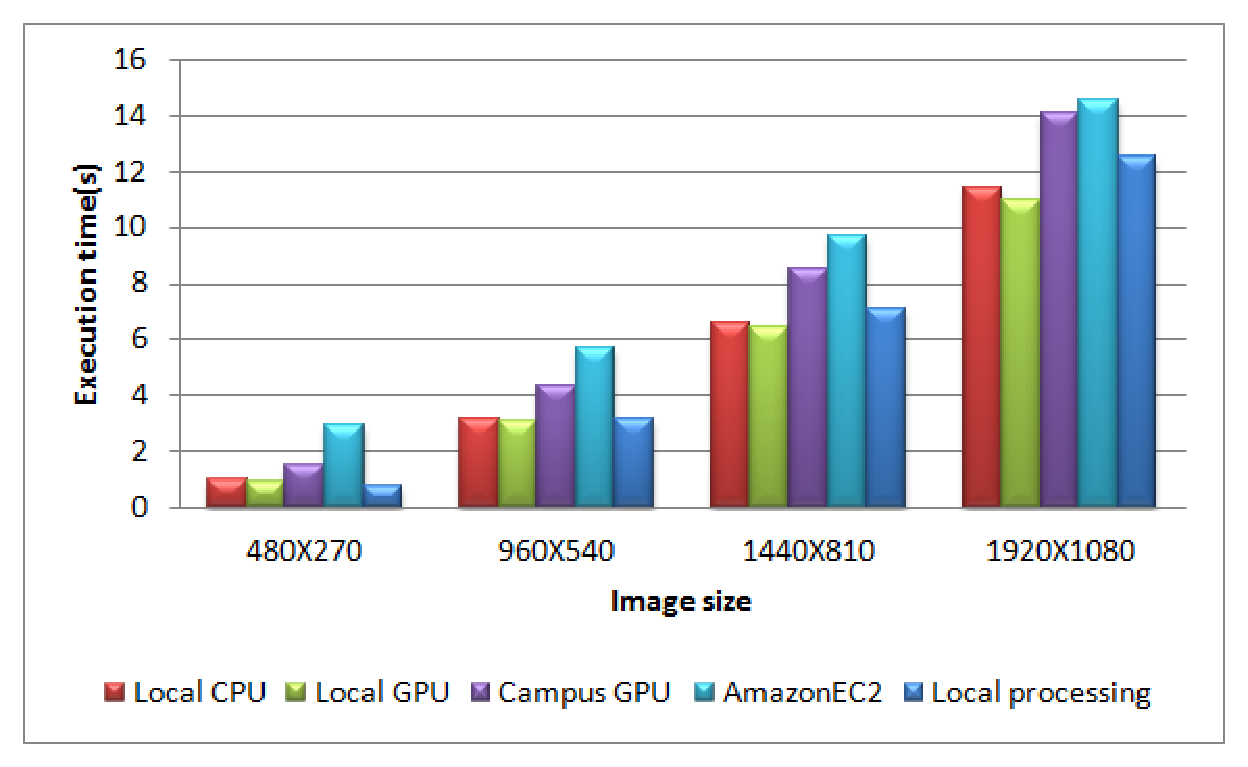
\includegraphics[height=4.5cm, width=7.3cm]{Figure/figure3-a.eps}} 
		\subfloat[Matrix multiplication]{\label{fig:figure3-b}
			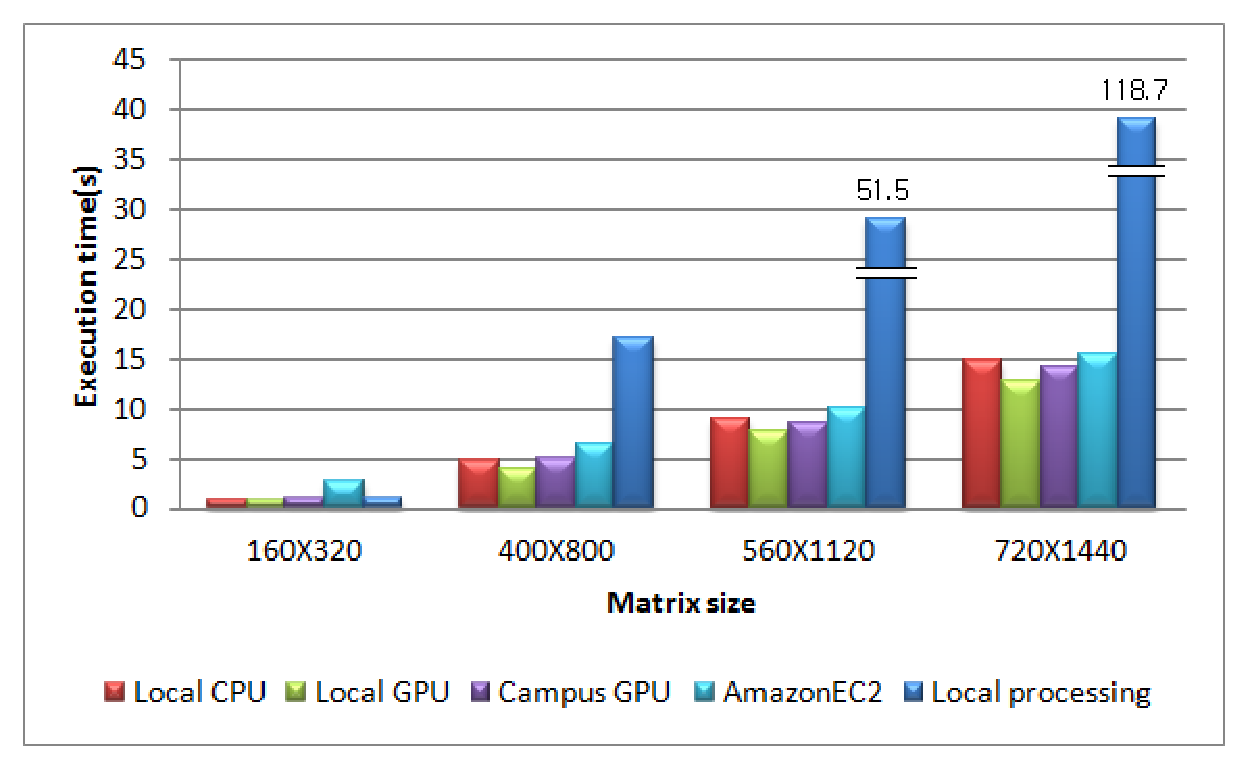
\includegraphics[height=4.5cm, width=7.3cm]{Figure/figure3-b.eps}}\\
		\subfloat[Hidden Markov mode]{\label{fig:figure3-c}
			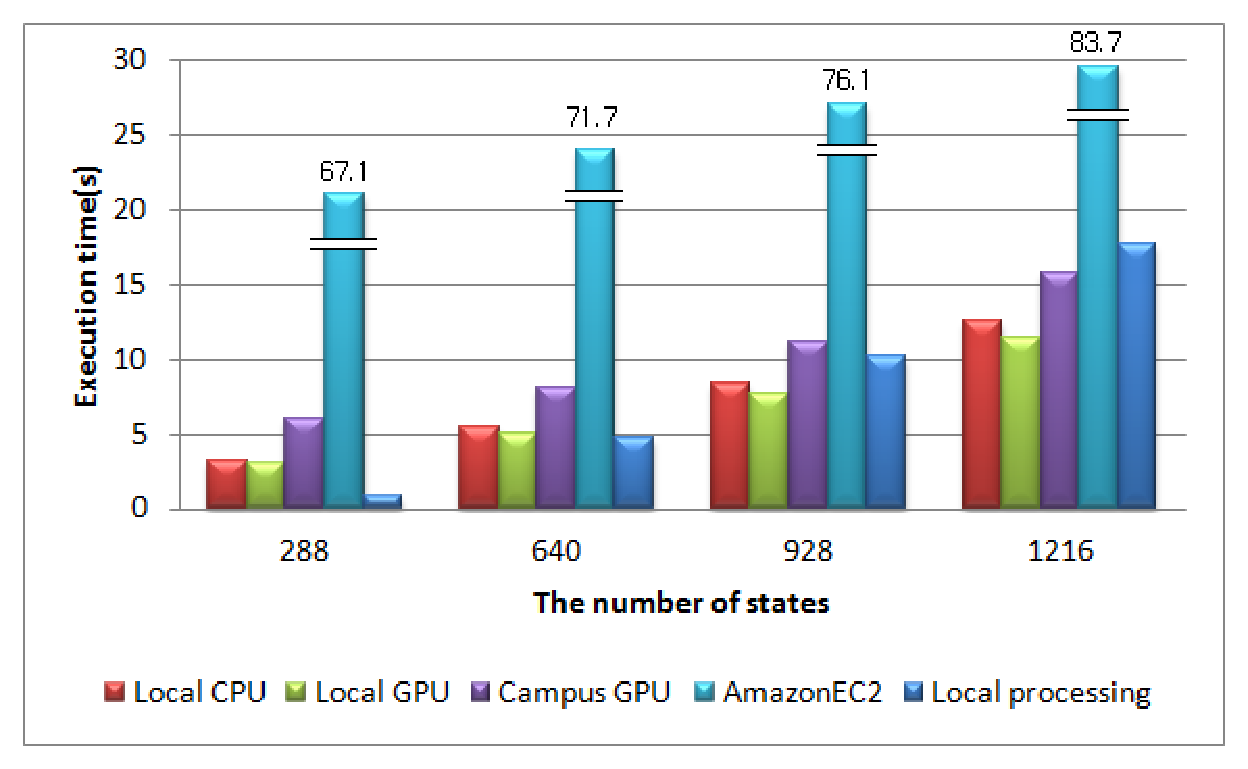
\includegraphics[height=4.5cm, width=7.3cm]{Figure/figure3-c.eps}}
		\subfloat[\textit{N}-body physics]{\label{fig:figure3-d}
			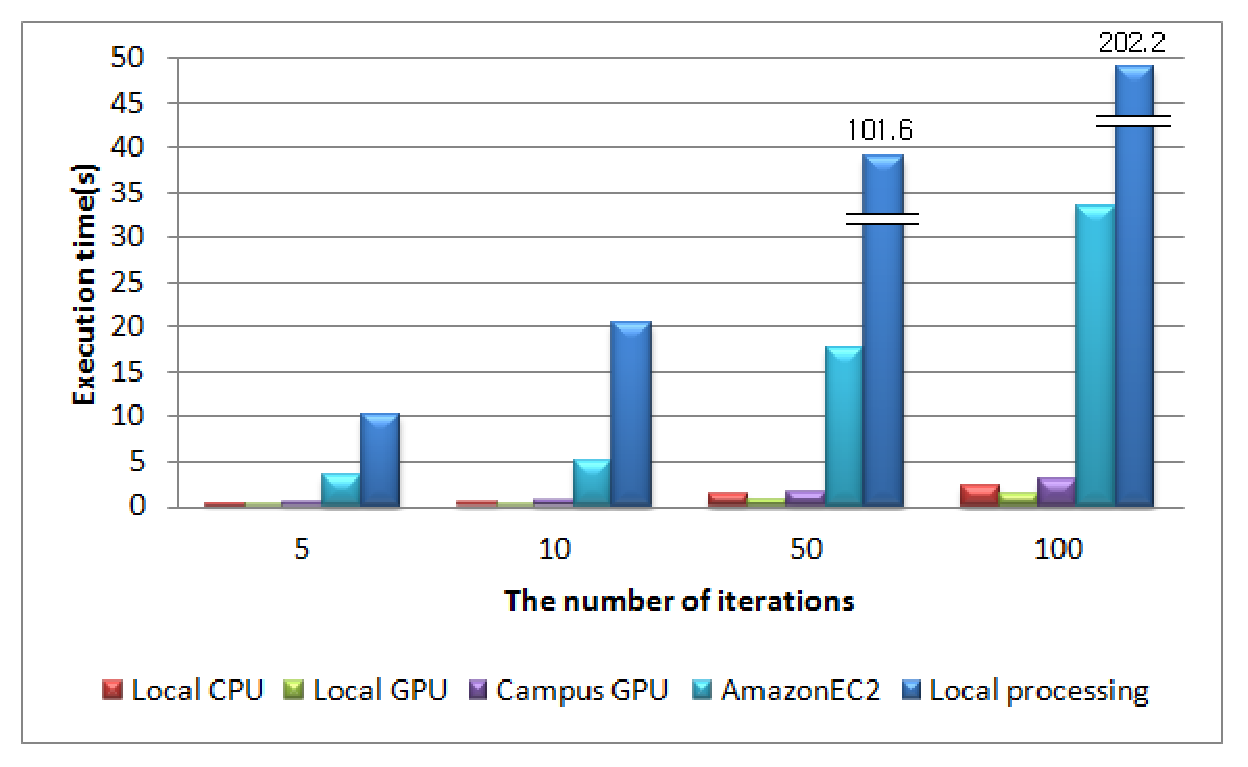
\includegraphics[height=4.5cm, width=7.3cm]{Figure/figure3-d.eps}}\\
	\end{tabular}
	\caption{Comparison of total execution time for four OpenCL
workloads with various servers and network setup}
\end{figure*}
%
\begin{figure*}
	\centering
	\begin{tabular}{c}
		\subfloat[Sobelfilter]{\label{fig:figure4-a}
			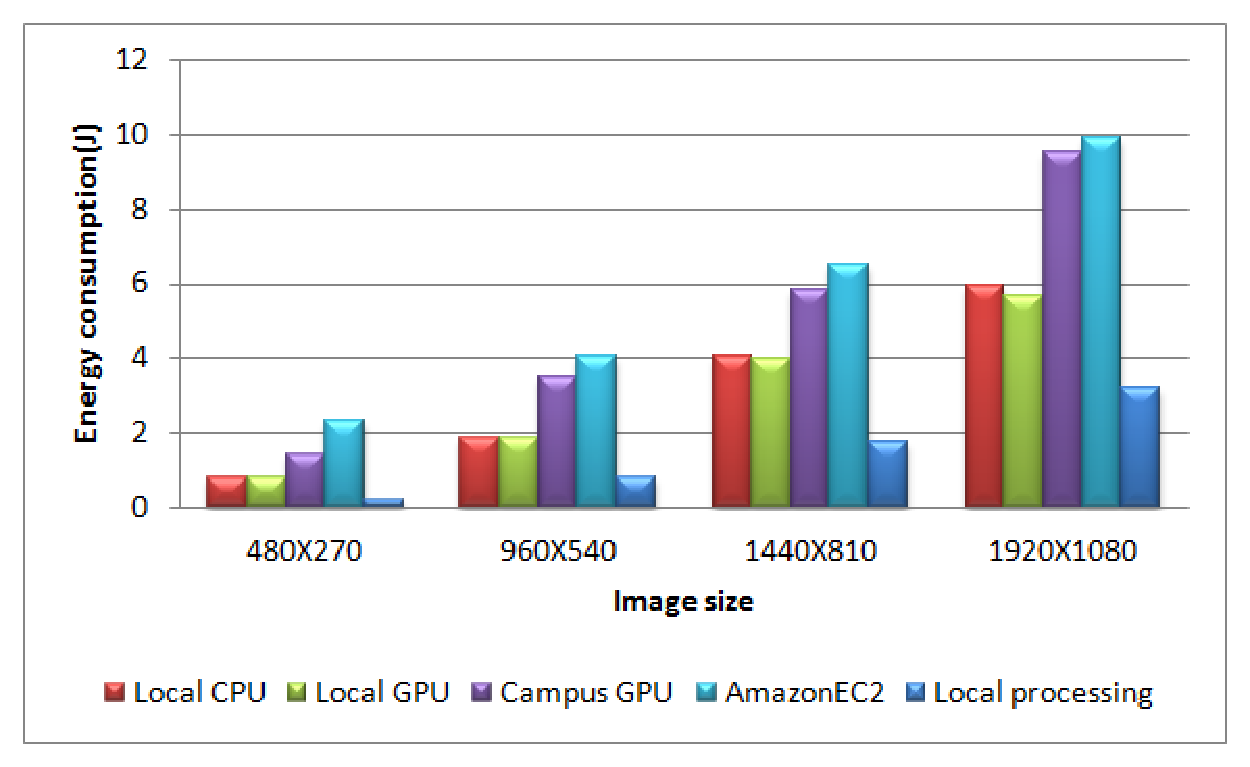
\includegraphics[height=4.5cm, width=7.3cm]{Figure/figure4-a.eps}} 
		\subfloat[Matrix multiplication]{\label{fig:figure4-b}
			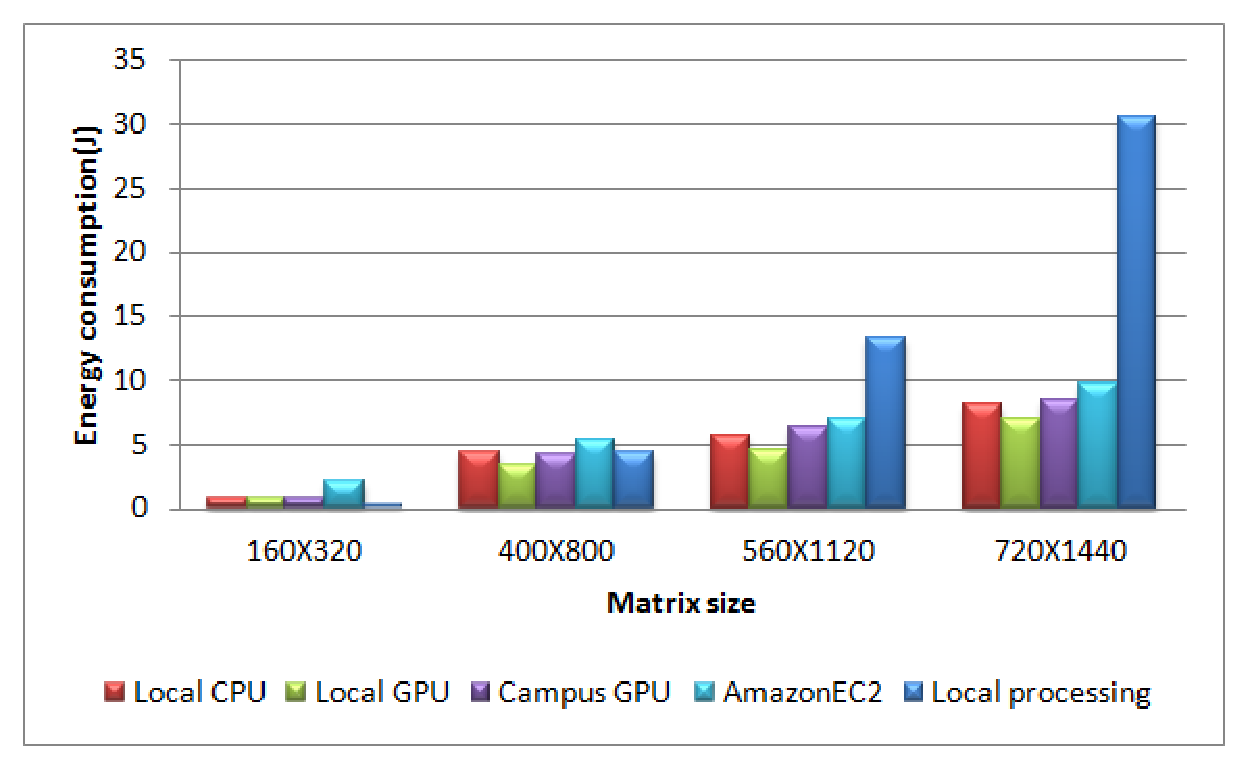
\includegraphics[height=4.5cm, width=7.3cm]{Figure/figure4-b.eps}}\\
		\subfloat[Hidden Markov mode]{\label{fig:figure4-c}
			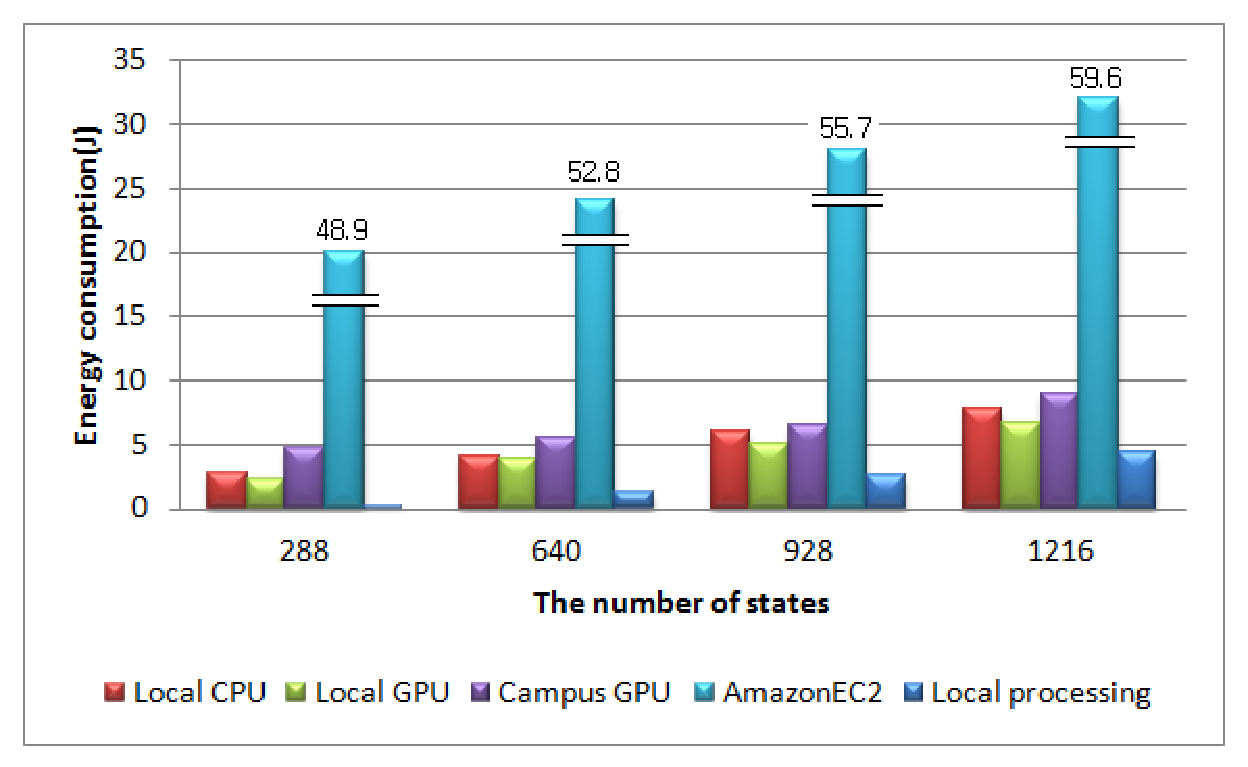
\includegraphics[height=4.5cm, width=7.3cm]{Figure/figure4-c.eps}}
		\subfloat[\textit{N}-body physics]{\label{fig:figure4-d}
			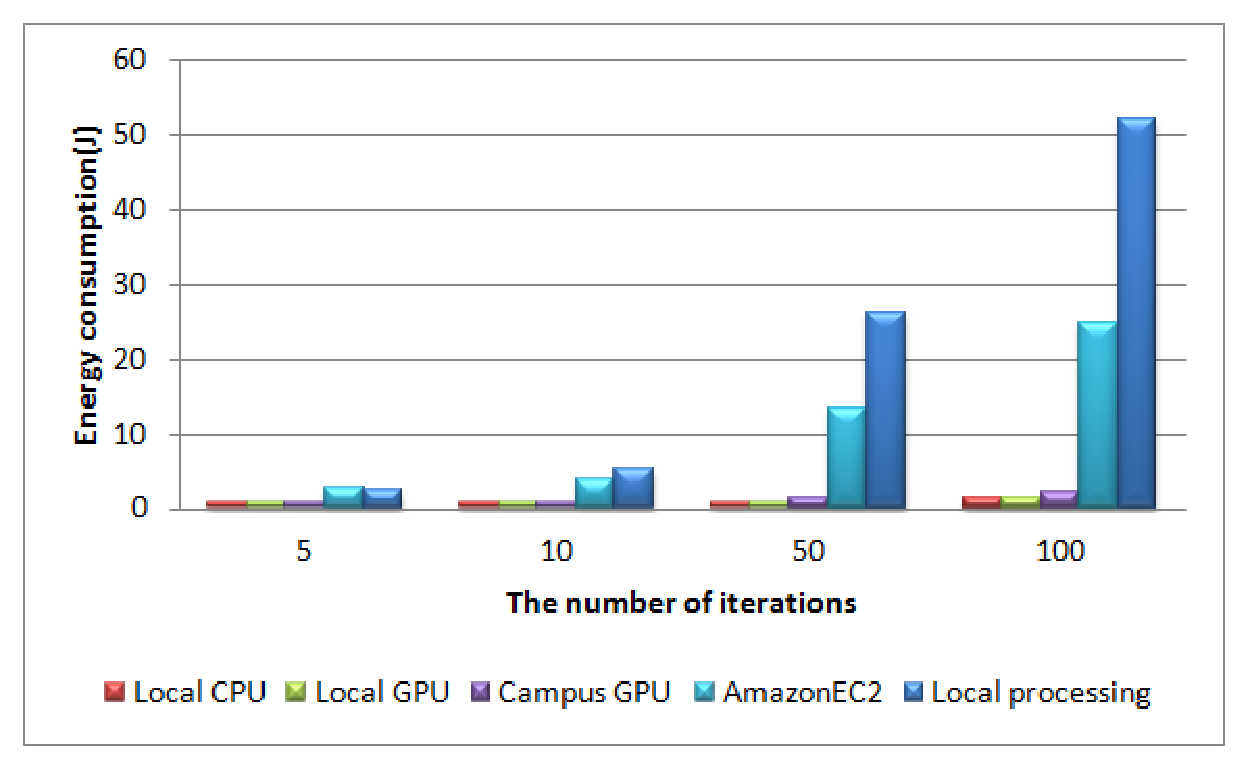
\includegraphics[height=4.5cm, width=7.3cm]{Figure/figure4-d.eps}}\\
	\end{tabular}
	\caption{Comparison of energy consumption for four OpenCL
workloads with various servers and network setup}
\end{figure*}
%
\subsection{Energy consumption}
To profile energy consumption of the mobile device, we used
PowerTutor~\cite{powertutor} which is an application for the variants of Android
devices that displays the power consumed by major components such as
GPU, network interfaces, LCD display, and GPS receiver.\\ 
%
\indent A similar pattern for energy consumption of the mobile device as
the execution time is shown in Figure 5.
%
As computation to communication value is higher, 
it is likely that offloading is more beneficial than local processing.
%
However, it is worth noting that though some cases for Sobelfilter
showed the benefits from offloading in terms of the execution time,
offloading consumes more than local processing as shown in Figure
3(a).
%
This dissimilar result comes from the discrepancy in the amount of power
consumed by CPU and the Wi-Fi networking card.
%
According to our measurement data profiled by PowerTutor, CPU consumes
200$\sim$220\textit{mW} per second in active mode, while the
Wi-Fi networking card consumes about 710$\sim$720\textit{mW}
per second in high power mode.
%
For that reason, even though offloading is faster than local processing,
it is possible that offloading consumes more energy than local
processing.
%
However, in matrix multiplication and \textit{N}-body physics which
result in extremely high speed-up by offloading, it is observed that
offloading also improves energy implication as shown in Figure 5(b) and
(d). 
%
\section{Related work}
\subsection{Mobile workload analysis}
In~\cite{fullsystem}, the authors characterize the microarchitectural
behavior of smartphone applications through several representative
benchmarks including the following areas: an interactive game, a
streaming player and mp3 audio player.
%
Also, they developed a new benchmark to characterize the performance 
of a web browser called BBench.
%
Through those benchmarks, they show how they differ from SPEC CPU2006
benchmarks which are widely used for the measurement of compute-intensive
performance.
%
MEVBench~\cite{mevbench} presented a custom benchmark suite for full mobile
vision applications such as augmented reality as well as components of
common vision algorithms such as SIFT feature extraction and SVM
classification.
%
The authors evaluated the performance of MEVBench with various
platforms for the direction of future mobile embedded vision
architectures.
%
Also, they show that mobile vision architectures require to be supported
from heterogeneous computation for performance improvement.
%
In~\cite{characterization}, the performance and energy benefits of
mobile heterogeneous computing are characterized by using 2D FFT(Fast
Fourier Transformation), matrix multiplication, and 2D Stencil as the
benchmarks.
%
In this study, the authors demonstrated that fully utilizing available
computing cores to complete a task can achieve an 3.7$\times$ speed-up
over the case of the single-threaded CPU, consequently, reduce the
energy consumption for the mobile platform.\\
%
\indent In contrast with the aforementioned studies which designed new
benchmarks or characterized the performance and energy benefits of
the mobile platforms via the various workloads from a perspective of
mobile computing capabilities, we characterized the behavior of mobile
offloading framework while considering the network conditions as well as
the computing capabilities of remote resources.
%
\subsection{Remote offloading framework}
The research community has proposed different methods to offload the
computation for the mobile platforms as well as high performance
clusters.
%
In Spectra~\cite{spectra}, developers identify functions in the
application that can be offloaded to a remote server over RPC.
%
By monitoring the CPU, file system, and bandwidth, Spectra dynamically
decides at run-time which portions of the application should run locally
or remotely.
%
MAUI~\cite{maui} takes a similar approach but alleviates the process by
using many of the programming features in the .NET platform such as
method attributes, and the Reflection API.
%
Through the .NET framework's virtual machine, MAUI is able to
dynamically serialize and ship remotable methods and data to a server
proxy.
%
Cuckoo~\cite{cuckoo} takes a slightly modified approach by focusing more on
integrating with the Eclipse IDE, however it requires developers to
implement both local and remote versions of their functionality, whereas
MAUI only requires annotations instead of a different implementation.
%
CloneCloud~\cite{clonecloud} achieves the remote offloading by employing thread
migration in the Dalvik Java virtual machine (JVM) by transferring all
of the thread state (thread stack, necessary heap objects and registers)
to the remote virtual machine.
%
When the remote thread completes, the results are merged back with the
local Dalvik JVM memory stack.
%
There also exist other heterogeneous offloading frameworks which are
similar to our approach.
%
Remote CUDA~\cite{rcuda} is one approach that extends the Nvidia CUDA API
to support remote offloading over the network.
%
Their goal is to minimize the network overhead and they analyze the
impact of using different networking technologies such as Gigabit
Ethernet or InfiniBand.
%
Virtual OpenCL~\cite{vocl} provides a similar solution which uses OpenCL
instead of the proprietary CUDA protocol.
%
They also focus on cluster environments but they leverage the MPI
library for memory and workload synchronization.\\
%
\indent Although we are not the first to propose the concept of offloading
heterogeneous workloads over the network, our design is the first to
consider this approach where offloading happens into mobile platforms.
%
Furthermore since our framework is designed for mobile platforms, it differs greatly
because it takes into account not only performance, but also power energy
consumption. 
%
\section{Conclusion}
In this paper, we analyzed the behavior of the mobile offloading
framework in terms of the offloading performance and energy implication
of the mobile devices with respect to characteristics of workloads and
environmental factors such as network conditions or the computing
capabilities of remote resources.
%
In order to characterize the workloads, we used computation to
communication ratio calculated by the local processing time divided by
the time for data transfer.
%
Furthermore, as part of the workload characterization effort, we
developed the OpenCL-based remote offloading framework by broadening the
scope of heterogeneity to include a new kind of platform component: the
computing capabilities on remote resources. 
%
We accomplish this by extending the well-defined hardware-level
offloading standard, OpenCL framework to support the various range of
remote computing elements over the network using the regular TCP/IP
network stack.
%
Also, we configured both local and wide area networks in which the
various computing capabilities are deployed to evaluate the impact of
environmental factors into the offloading performance.
%
According to the analysis, the benefits and the costs of the remote
offloading depend on computation to communication ratio as well as the
programming flow related to how the client and the server interact each
other.
%
In fact, as computation to communication ratio becomes higher, 
the performance improvement and the conservation of energy consumption 
also increase.
%
Moreover, in the cases of hidden Markov model and \textit{N}-body
physics, we observed that the programming flow is also important to
analyze the behavior of the remote offloading for the mobile
platforms.  
%
We believe that the numerical results presented in this paper guides the basis
of designing the intelligent runtime offloading scheduler, so we are
currently working on a machine learning-based runtime offloading scheduler.
%
Also, we are currently seeking to real mobile applications such as face and
voice recognition, or mobile gaming so that we are able to 
evaluate the proposed offloading framework with those
applications.
%
\section*{Acknowledgment}
This material is based upon work supported by the National Science
Foundation under Grant No. 0758596.
%
Any opinions, findings, and conclusions or recommendations expressed in
this material are those of the author(s) and do not necessarily reflect
the views of the National Science Foundation.
%
\bibliography{IISWC13}

%\begin{thebibliography}{1}

%\bibitem{IEEEhowto:kopka}
%H.~Kopka and P.~W. Daly, \emph{A Guide to \LaTeX}, 3rd~ed.\hskip 1em plus
%  0.5em minus 0.4em\relax Harlow, England: Addison-Wesley, 1999.

%\end{thebibliography}

% that's all folks
\end{document}


